\documentclass[10pt,pdf,utf8,russian,aspectratio=169]{beamer}
\usepackage[T2A]{fontenc}
\usepackage[english,russian]{babel}
\usepackage{float}
\usepackage[normalem]{ulem}

\usetheme{metropolis}   

\usepackage{booktabs}
\usepackage[scale=2]{ccicons}


\usepackage{pgfplots}
\usepgfplotslibrary{dateplot}

\definecolor{BI}{RGB}{63,143,213}
\setbeamercolor{frametitle}{bg=BI}
\setbeamercolor{title separator}{fg=BI}
\setbeamercolor{progress bar in section page}{fg=BI}

\title{GeneQuery}
\subtitle{Система поиска фенотипов}
\date{\today}
\author{Арбузов Иван}
\institute{Институт Биоинформатики}
\titlegraphic{\hfill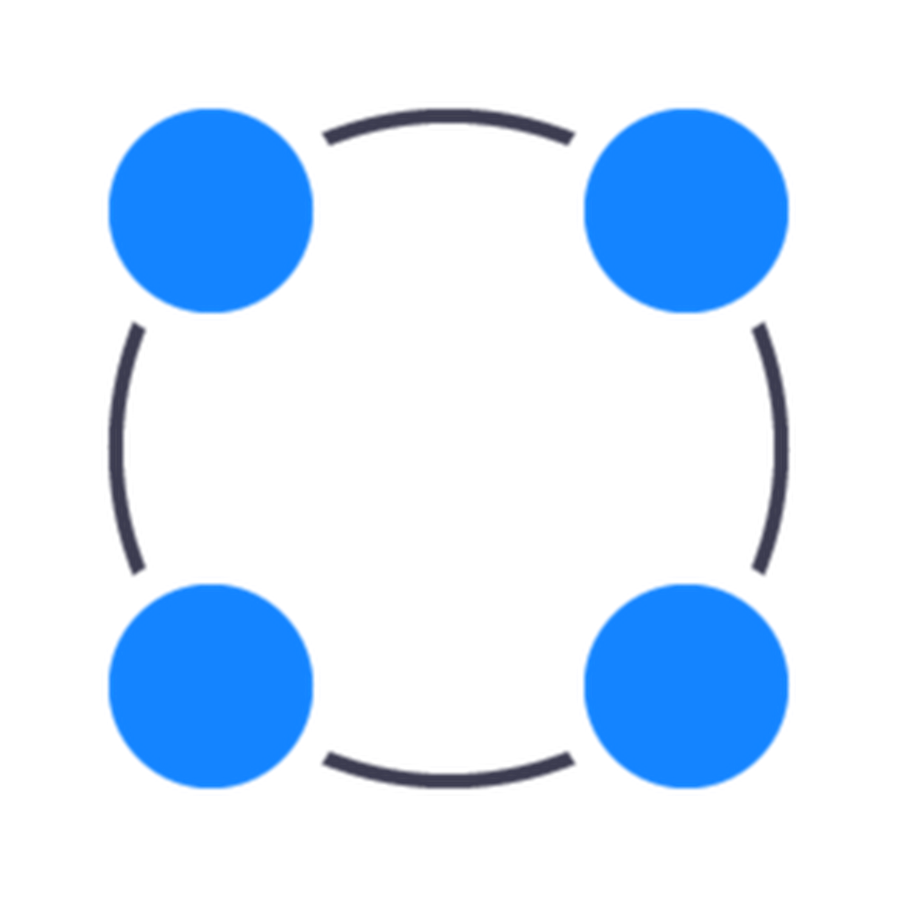
\includegraphics[height=1.5cm]{logo}}

\begin{document}

\maketitle

\begin{frame}
  \frametitle{Содержание}
  \setbeamertemplate{section in toc}[sections numbered]
  \tableofcontents
\end{frame}

\section{Введение в поиск фенотипов}

\begin{frame}{Описание проблемы}
  \begin{itemize}[<+->]
    \item Провели эксперимент
    \item Получили набор «проявивших» себя генов
    \item \alert{Как проинтерпретировать результат?}
  \end{itemize}
\end{frame}

\begin{frame}{Интерпретация результата}
  \begin{itemize}[<+->]
    \item Экспертная интерпретация
    \item Лексический анализ (текстов, статей и т.д.)
    \item \alert<4> {Аналитическая интерпретация (статистика, теория вероятностей и т.д.)}
  \end{itemize}
\end{frame}

\begin{frame}{Общая постановка задачи}
  \begin{itemize}[<+->]
    \item Имеется множество результатов (наборов одинаково регулируемых генов) уже проделанных экспериментов
    \item Имеется результат (набор генов) нового эксперимента
    \item Найти среди уже сделанных экспериментов те, в которых гены ведут себя \alert<4>{«похожим»} образом
  \end{itemize}
\end{frame}


\section{GeneQuery: обзор}

\begin{frame}{Используемые данные}
  \begin{itemize}[<+->]
    \item Основан на базе данных GEO
    \item Датасет содержит информацию об экспрессии генов $k$ образцов, участвовавших в эксперименте
    \item 6000 наиболее «активных» генов разбиты на кластеры алгоритмом WGCNA
    \item Pathway экспрессий генов одного кластера \emph{совпадает} (up-/down-regulated)
  \end{itemize}
\end{frame}

\begin{frame}{Кластеры}
    \begin{figure}[p]
        \centering
        \caption{Теплокарта кластеров эксперимента}
        \includegraphics[height=0.8\textheight]{./img/clasters.png}
    \end{figure}      
\end{frame}

\begin{frame}{Используемые данные}
  \begin{itemize}[<+->]
    \item Произвели поиск по GEO (от 8 до 100 образцов в эксперименте, microarray)
    \item Выкачали GPL, отфильтровали по ряду принзнаков (частота встречаемости)
    \item Выкачали все GSE для оставшихся GPL
    \item Preprocessing (лог-нормализация, sanity checks)
    \item 3k для мышей, 3.8k для человека
    \item $\sim$ 50k кластеров для мышки, $\sim$ 80k --- для человека
  \end{itemize}
\end{frame}

\begin{frame}{Архитектура}
    \begin{figure}[p]
        \centering
        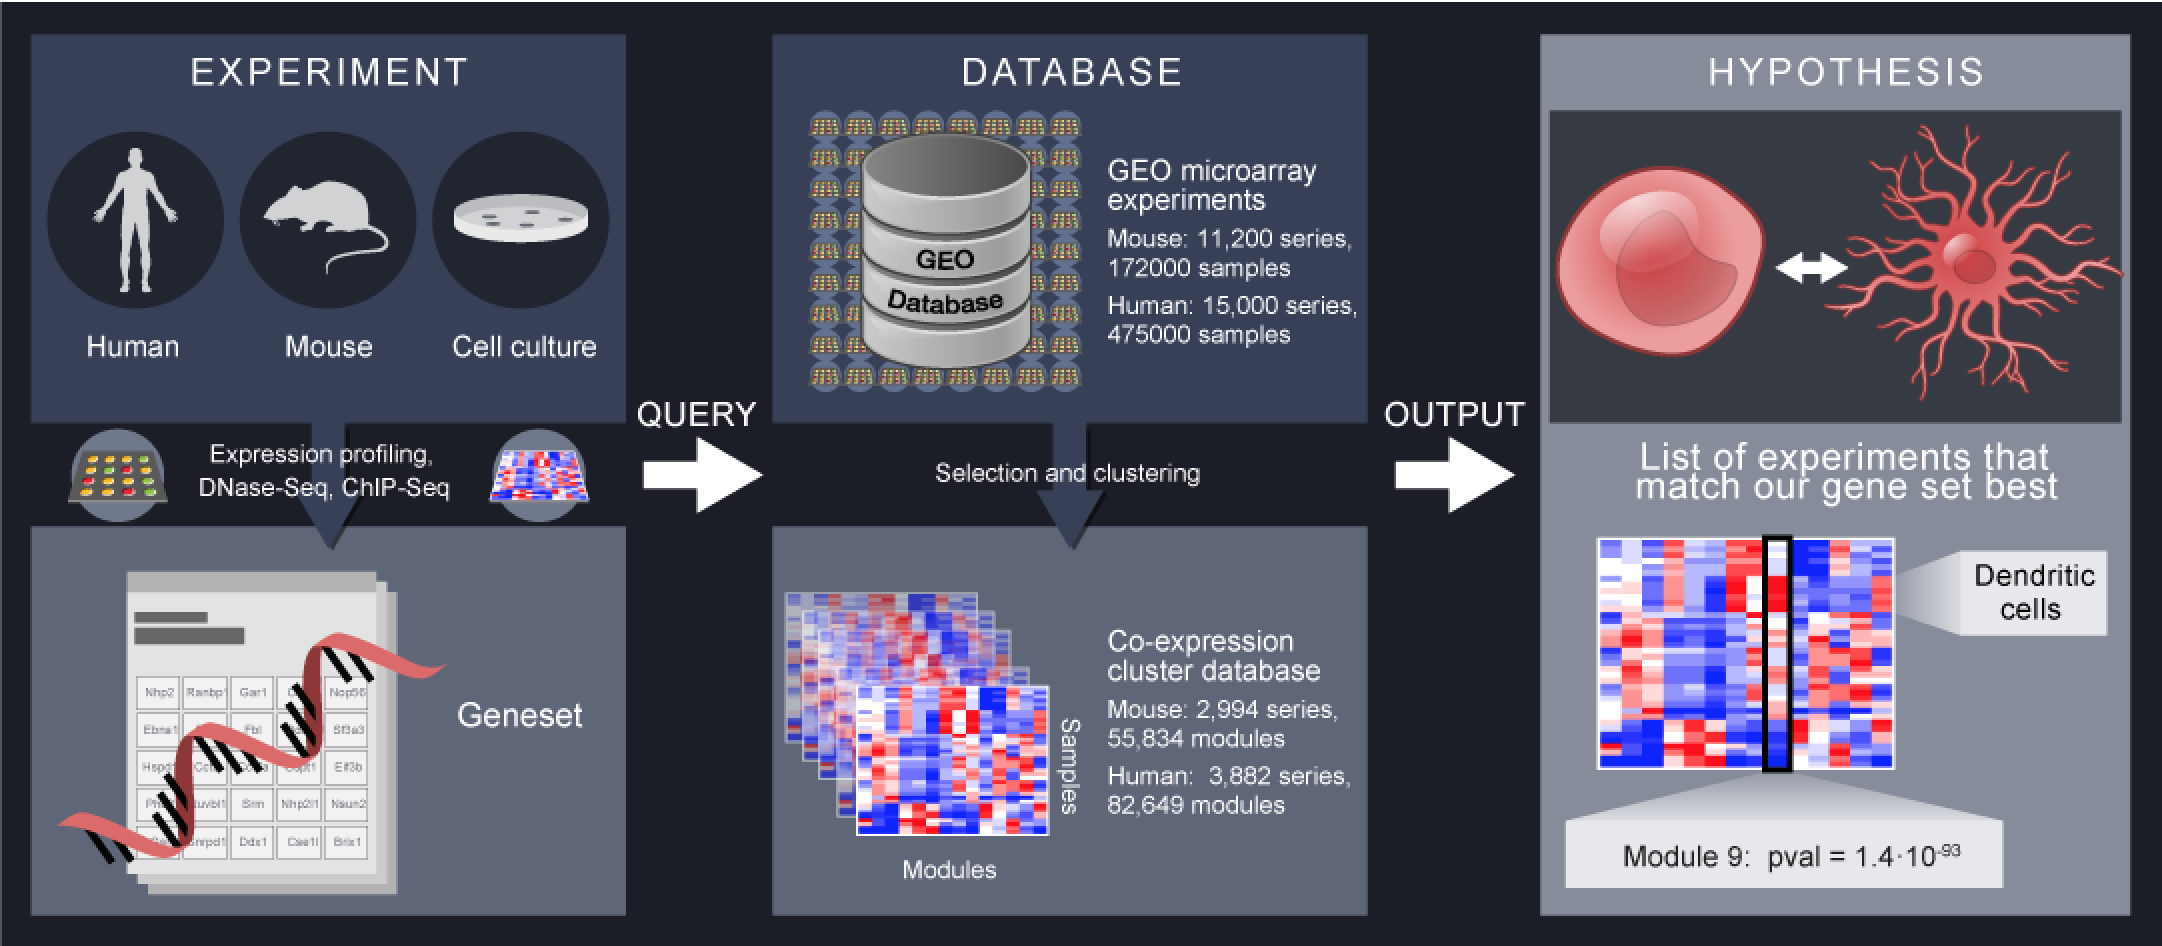
\includegraphics[width=0.9\textwidth]{./img/architecture.png}
    \end{figure}      
\end{frame}

\begin{frame}
    \begin{figure}[p]
        \centering
        \caption{Форма запроса.}
        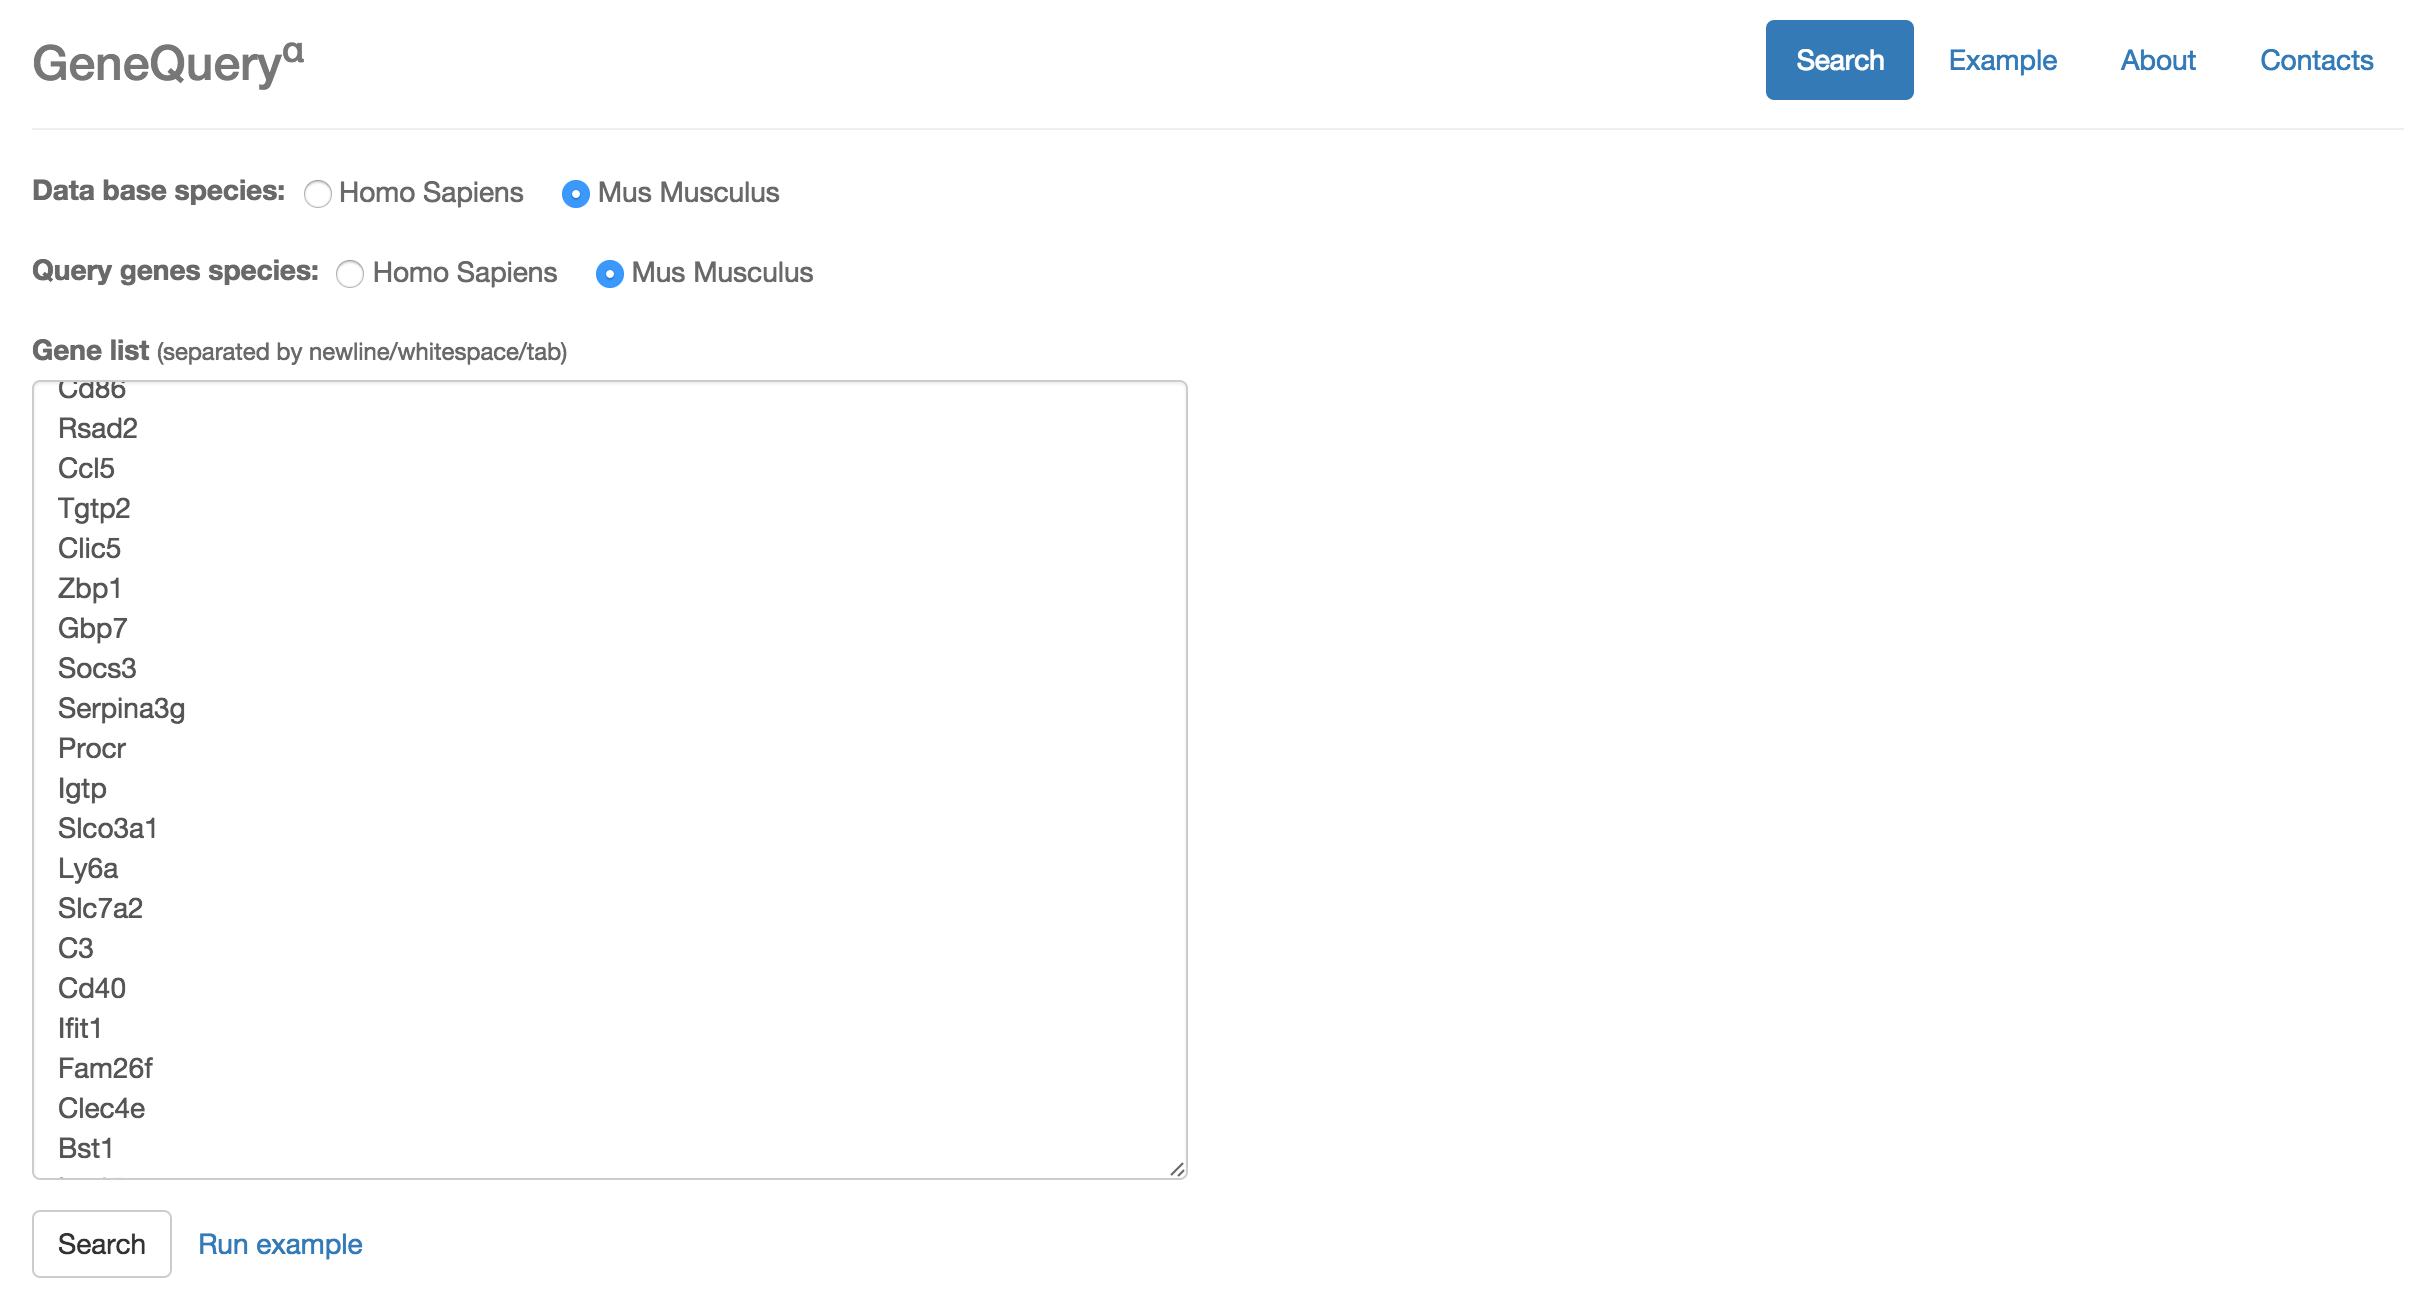
\includegraphics[height=0.9\textheight]{./img/screen_query.png}
    \end{figure}
\end{frame}

\begin{frame}
    \begin{figure}[p]
        \centering
        \caption{Таблица с результатами.}
        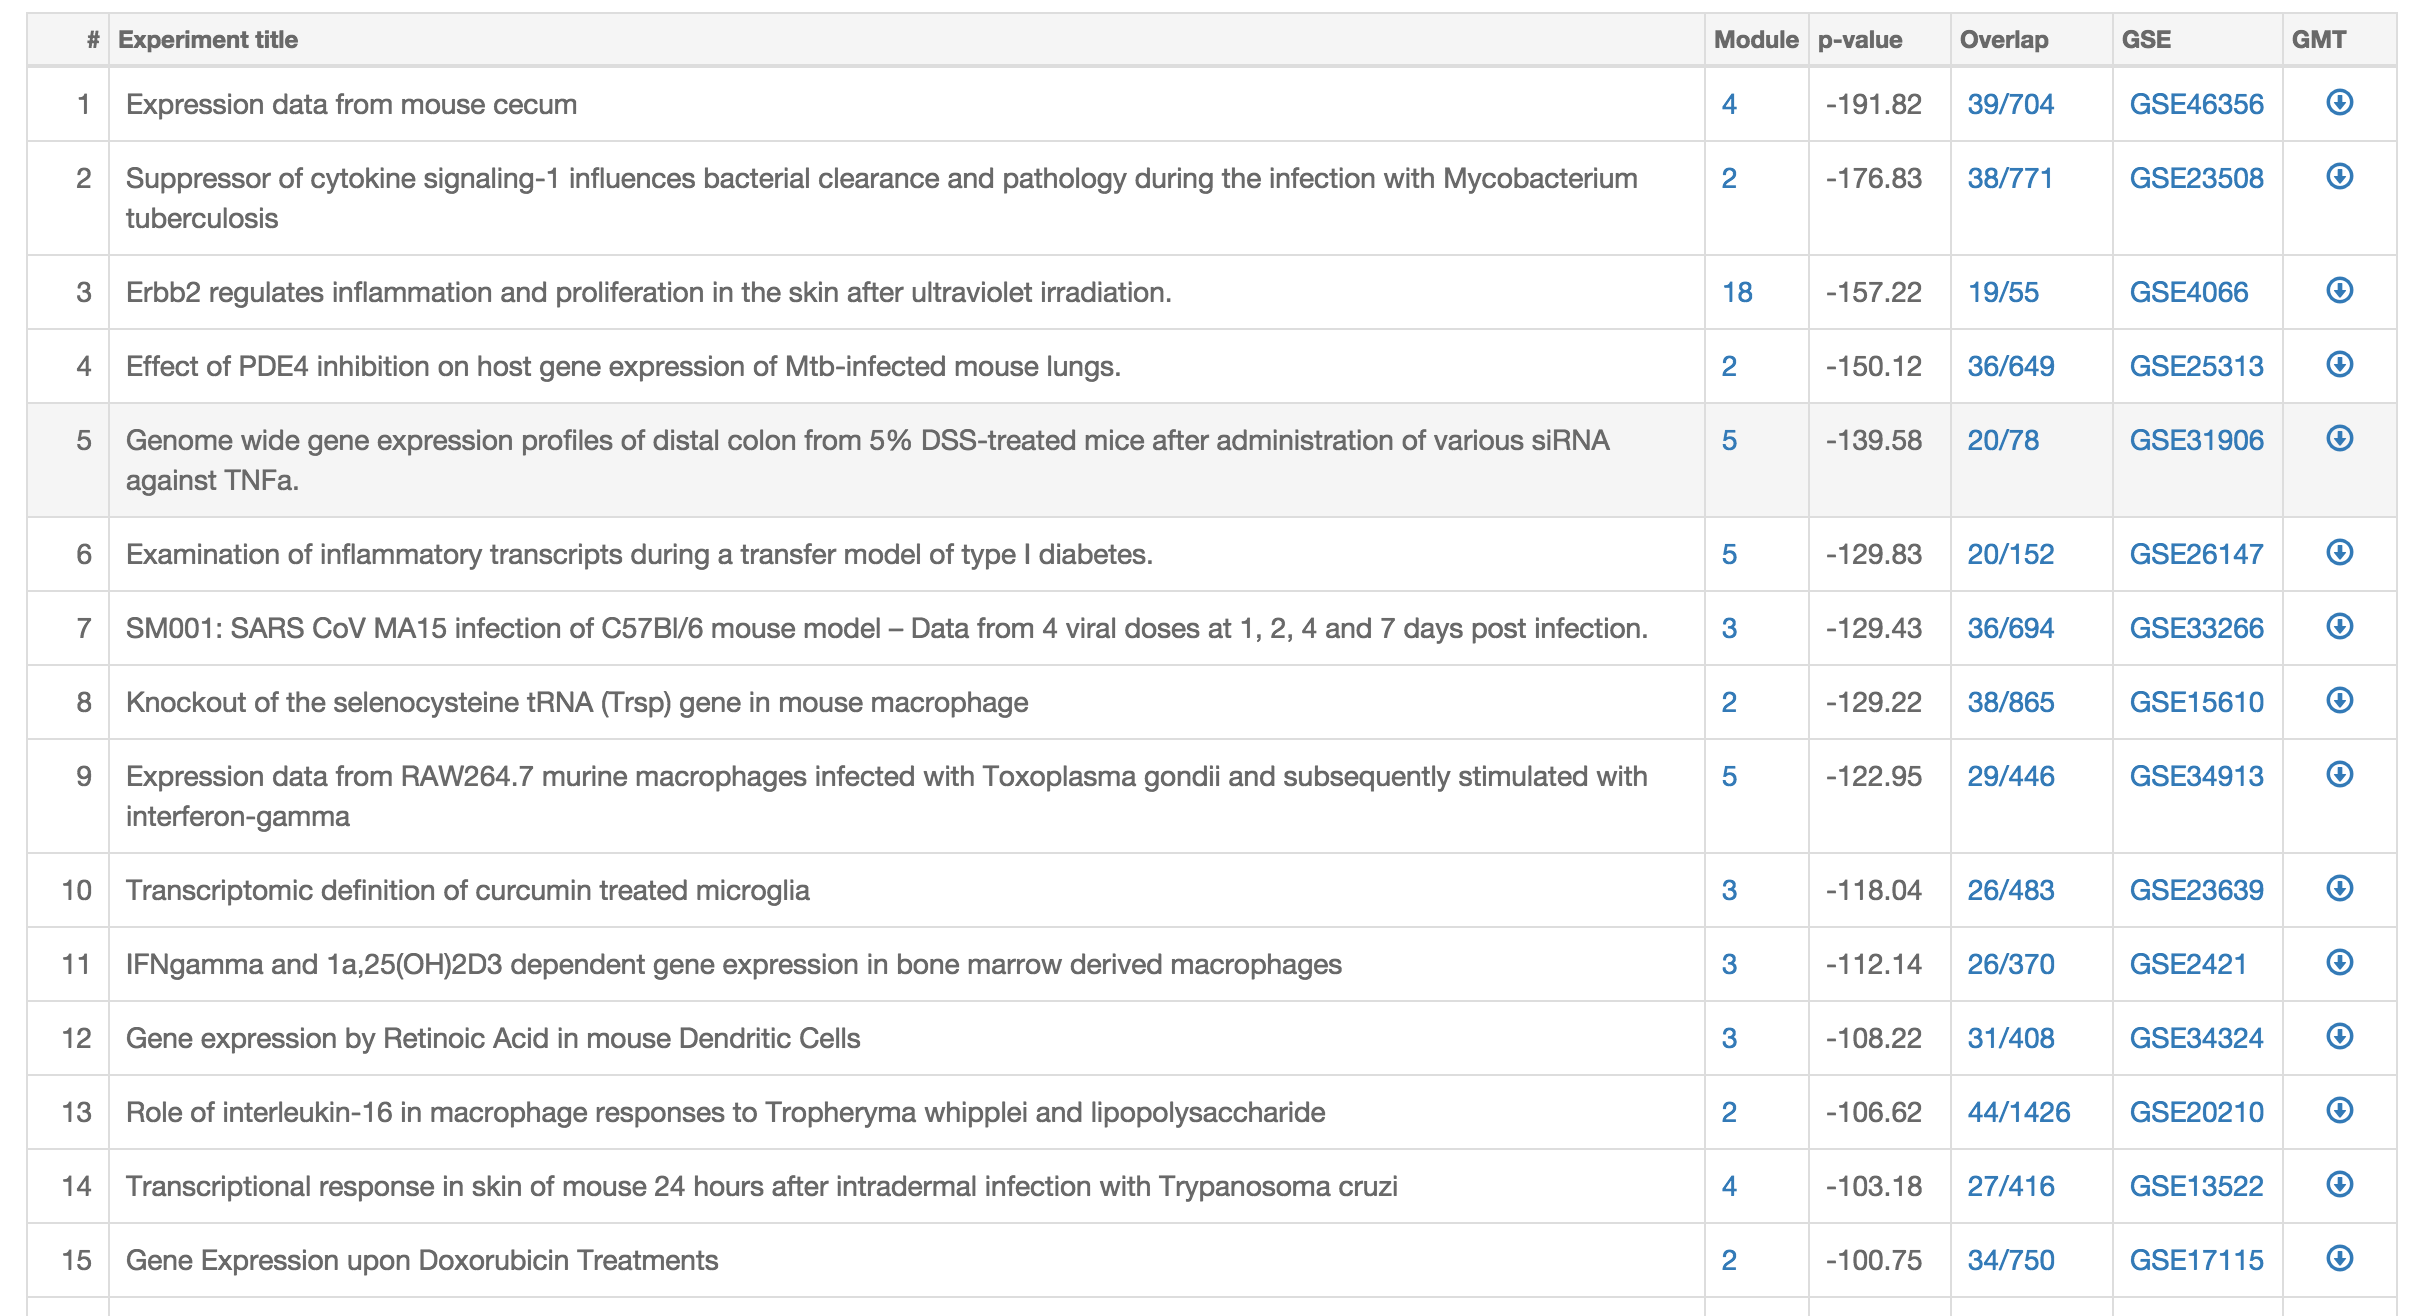
\includegraphics[height=0.9\textheight]{./img/screen_results.png}
    \end{figure}
\end{frame}

\begin{frame}
    \begin{figure}[p]
        \centering
        \caption{Детализация конвертации генов.}
        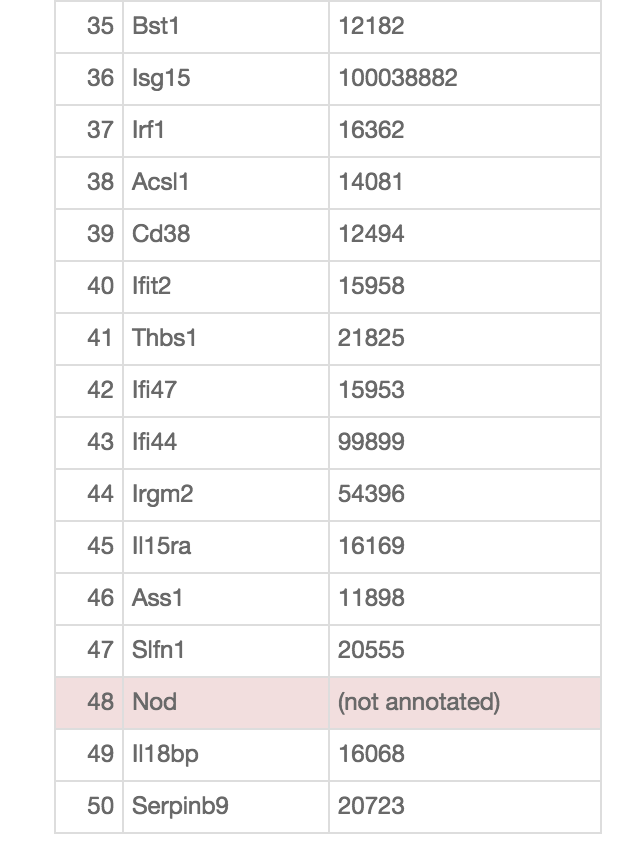
\includegraphics[height=0.9\textheight]{./img/screen_details.png}
    \end{figure}
\end{frame}

\begin{frame}
    \begin{figure}[p]
        \centering
        \caption{Heatmap.}
        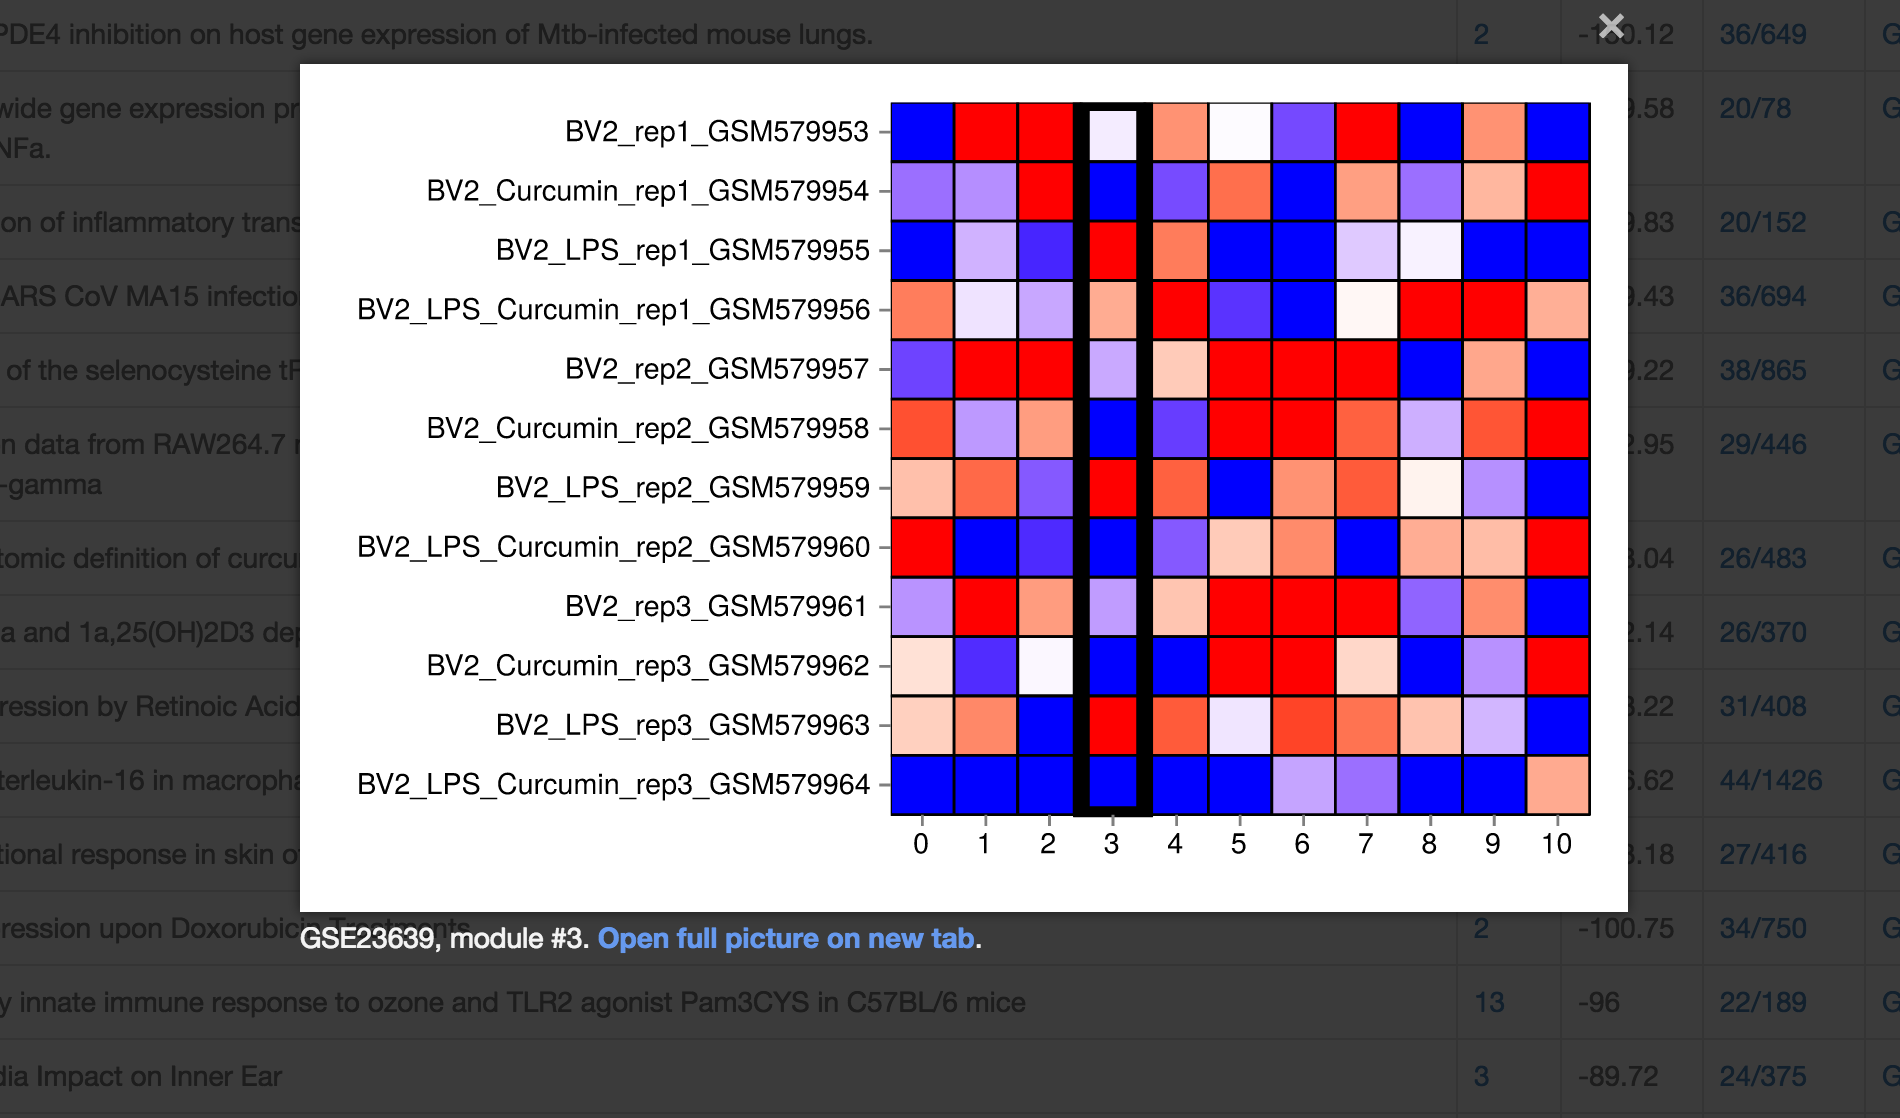
\includegraphics[height=0.9\textheight]{./img/screen_heat.png}
    \end{figure}
\end{frame}

\begin{frame}
    \begin{figure}[p]
        \centering
        \caption{Гены из пересечения в Symbol нотации.}
        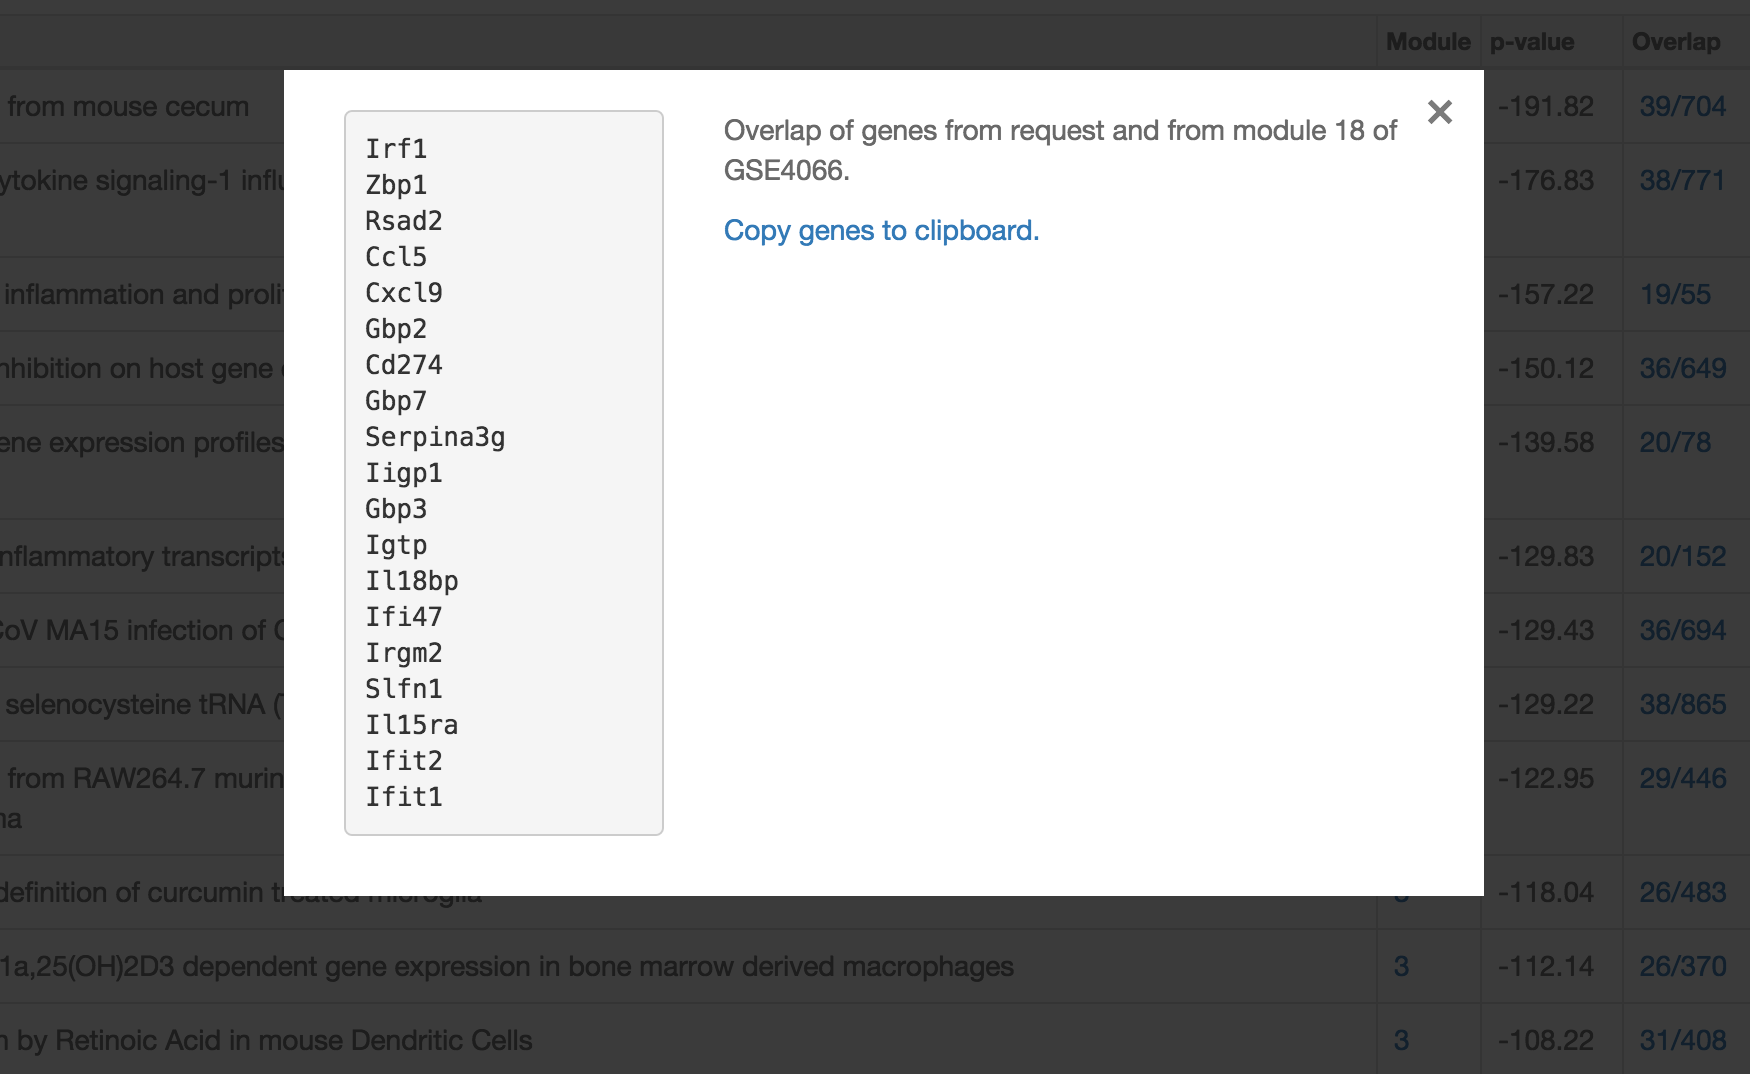
\includegraphics[height=0.9\textheight]{./img/screen_overlap.png}
    \end{figure}
\end{frame}


\section{GeneQuery: под капотом}

\subsection{Вероятностная модель}

\begin{frame}{Условности}
  \begin{itemize}[<+->]
    \item Ген уникально идентифицируется своим \emph{Entrez ID} --- неким натуральным числом
    \item Запрос --- набор генов ненулевого размера
    \item Модуль --- кластер после работы алгоритма WGCNA
    \item GSE --- все кластеры какого-либо эксперимента (с $k$ образцами)
  \end{itemize}
\end{frame}

\begin{frame}{Пересечение запроса и модуля}
  \begin{itemize}[<+->]
    \item Пусть имеется некоторый набор генов (запрос)
    \item Зафиксируем какой-либо модуль из нашей базы данных
    \item Найдем пересечение запроса и модуля
    \begin{figure}[ht]
        \centering
        \includegraphics[height=0.5\textheight]{./img/venn.png}
    \end{figure}
    \item \emph{Какова вероятность получить получить именно такое пересечение?}
    \item Гипергеометрическое распределение
  \end{itemize}
\end{frame}

\begin{frame}{Понимаем гипергеометрическое распределение}
  \begin{itemize}[<+->]
    \item Пусть имеется урна с $N$ шариками двух цветов: $D$ белых, $N - D$ черных
    \item Вытянем из урны $n$ шаров одновременно
    \item Какова вероятность, что $k$ из $n$ шаров окажутся белыми?
  \end{itemize}
\end{frame}

\begin{frame}{Точная формула вероятности}
    \begin{block}{Вероятность вытянуть $k$ белых шаров}
        \begin{equation}
        f(k; N, D, n) = \frac{\binom{D}{k}\binom{N - D}{n - k}}{\binom{N}{n}}
        \end{equation},
        где $N$ --- шаров в урне,
            $D$ --- белых шаров в урне,
            $n$ --- количество вытянутых шаров,
            $k$ --- количество вытянутых \emph{белых} шаров.
    \end{block}
\end{frame}

\begin{frame}{Сведение к гипергеометрическому распределению}
  \begin{itemize}[<+->]
    \item Пусть $N$ --- множество всех генов GSE ($\sim 6000$), $D$ --- множество генов в запросе
    \item «Покрасим» в белый цвет те гены из $N$, которые присутствуют и в $D$
    \item Пусть $n$ --- какой-либо модуль из данного GSE
    \item \emph{Какова вероятность, что $k$ генов из этого модуля «покрашены» в белый цвет, т.е. принадлежат множеству генов из запроса?}
  \end{itemize}
\end{frame}

\begin{frame}{Точная формула вероятности}
    \begin{block}{Вероятность иметь $k$ генов из запроса в модуле $n$}
        \begin{equation}
        f(k; N, D, n) = \frac{\binom{D}{k}\binom{N - D}{n - k}}{\binom{N}{n}}
        \end{equation},
        где $N$ --- количество генов в GSE, которому принадлежит модуль $n$,
            $D$ --- количество генов в запросе,
            $n$ --- количество генов в модуле,
            $k$ --- количество генов в пересечении модуля и запроса.
    \end{block}
\end{frame}

\begin{frame}{Оценка значимости пересечения}
  \begin{itemize}[<+->]
    \item На сколько данное пересечение статистически значимо?
    \item Точный тест Фишера
  \end{itemize}
\end{frame}

\begin{frame}{Точный тест Фишера}
    Рассмотрим таблицу
    \begin{table}[!ht]
        \centering
        \begin{tabular}{c|c|c|c}
                 & Юноши   & Девушки &  Всего \\ \hline
        на диете & $a$     & $b$     & $a + b$ \\ \hline
     не на диете & $c$     & $d$     & $c + d$ \\ \hline
           всего & $a + c$ & $b + d$ & $n$ \\
        \end{tabular}
    \end{table}
    Вероятность того, что $a$ юношей не на диете, вычисляется по формуле гипергеометрического распределения:
        $$\mathsf{Pr}(a) = \frac{\binom{a + b}{a}\binom{c + d}{c}}{\binom{n}{a + c}}$$
\end{frame}

\begin{frame}{Точный тест Фишера: пример}
    Рассмотрим таблицу
    \begin{table}[!ht]
        \centering
        \begin{tabular}{c|c|c|c}
                 & Юноши   & Девушки &  Всего \\ \hline
        на диете & $1$     & $9$     & $10$ \\ \hline
     не на диете & $11$     & $3$     & $14$ \\ \hline
           всего & $12$ & $12$ & $24$ \\
        \end{tabular}
    \end{table}
    \onslide<2->{Какова вероятность, что из 12 юношей лишь один будет на диете?} \\
    \onslide<3>{Правда ли, что склонность к диете не зависит от пола?}
\end{frame}

\begin{frame}{Точный тест Фишера}
  \begin{itemize}[<+->]
    \item Нулевая гипотеза: \emph{склонность к диете не зависит от пола}
    \item Посчитаем вероятность получить такое или более \emph{«перекошенное»} (при одинаковой сумме в строках и столбцах) распределение юношей
    \item Эта вероятность --- статистическая значимость наблюдения
  \end{itemize}
\end{frame}

\begin{frame}{Точный тест Фишера: пример}
    В нашем примере только одна таблица более перекошена:
    \begin{table}[!ht]
        \centering
        \begin{tabular}{c|c|c|c}
                 & Юноши   & Девушки &  Всего \\ \hline
        на диете & $0$     & $10$     & $10$ \\ \hline
     не на диете & $12$     & $2$     & $14$ \\ \hline
           всего & $12$ & $12$ & $24$ \\
        \end{tabular}
    \end{table}
    \onslide<2->{
        Результирующая значимость будет вычисляться:
        $$p_{value} = \mathsf{Pr}(1) + \mathsf{Pr}(0)$$
    }
    \onslide<3->\emph{
        При выполнении нулевой гипотезы вероятность получить исходную таблицу равна $p_{value}$
    }
\end{frame}

\begin{frame}{Применение теста Фишера}
    Для оценки статистической значимости пересечения запроса с модулем используется таблица:
     \begin{table}[!ht]
        \centering
        \begin{tabular}{c|c|c|c}
                 & пересек. с GSE & не пересек.с GSE & Всего \\  \hline
        в модуле & $k$            & $n - k$          & $n$ \\ \hline
     не в модуле & $D - k$        & $N - D + k - n$  & $N - n$ \\ \hline
           всего & $D$            & $N - D$          & $N$ \\
        \end{tabular}
    \end{table}
    \onslide<2->{
        Результирующая значимость получается по формуле:  
        $$ p_{value} = \sum_{i = k}^{min(D, n)} \mathsf{Pr}(i) $$
        т.н. \emph{правосторонний} тест Фишера.
    }
\end{frame}

\begin{frame}{Проблема множественных сравнений}
  \begin{itemize}[<+->]
    \item Статистический тест дает точный результат при \emph{одном} испытании
    \item При увеличении количества испытаний вероятность \emph{случайно} получить низкий $p_{value}$ (т.е. значимый результат) возрастает
    \item Поправка Бонферрони решает проблему, но грубо:
    $$\hat{p_i} = p_i \cdot m$$, где $m$ --- количество испытаний, $p_i$ --- значимость результата $i$-го испытания, $\hat{p_i}$ --- новая значимость
  \end{itemize}
\end{frame}

\subsection{Bootstrapping}

\begin{frame}{Множественные сравнения в GeneQuery}
  \begin{itemize}[<+->]
    \item Рассмотрим, как устроены данные в GeneQuery
    \item Далее под $p_{value}$ понимается минимальное $p_{value}$ среди всех модулей для конкретного вида (человек или мышь)
  \end{itemize}
\end{frame}
   
   
\begin{frame}
    \begin{figure}[p]
        \centering
        \caption{Распределение $log(p_{value})$ для запросов из 500 генов. Человек.}
        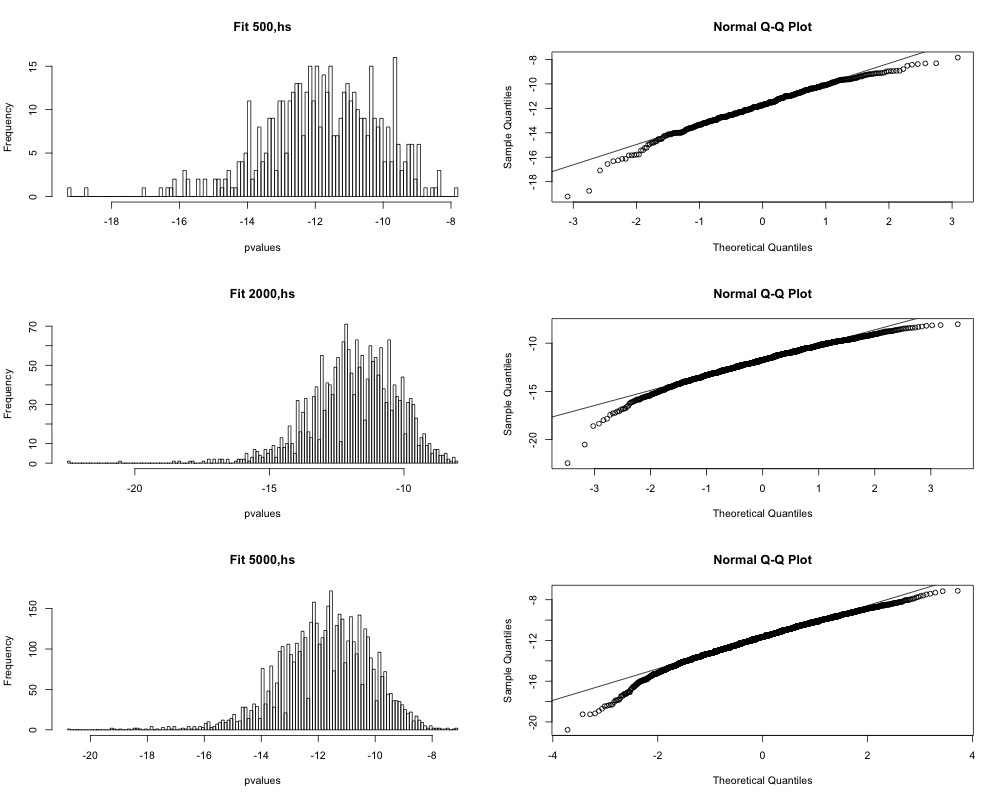
\includegraphics[height=0.95\textheight]{./img/converge_to_norm_query_size_500_hs.jpeg}
    \end{figure}
\end{frame}

\begin{frame}
    \begin{figure}[!ht]
        \centering
        \caption{Распределение $log(p_{value})$ для запросов из 25, 250, 2500 генов.}
        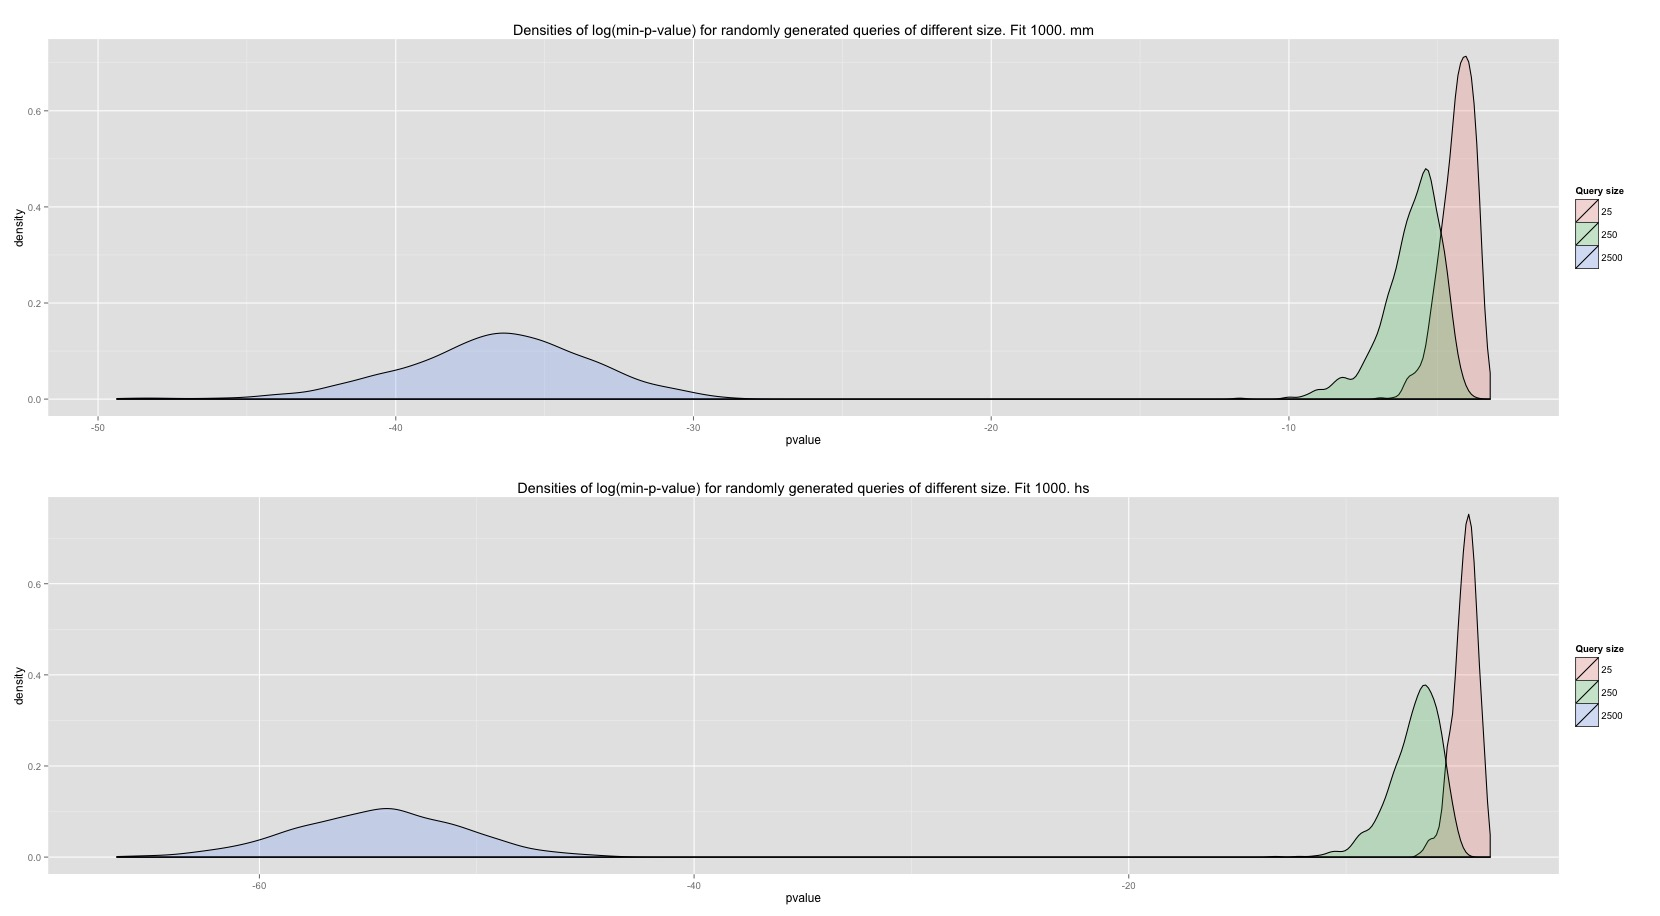
\includegraphics[width=\textwidth]{./img/densities_size_25_25_2500_fit_1000.jpeg}
    \end{figure}
\end{frame}

\begin{frame}
    \begin{figure}[!ht]
        \centering
        \caption{Регрессия $mean(log(p_{value}))$ от длины запроса.}
        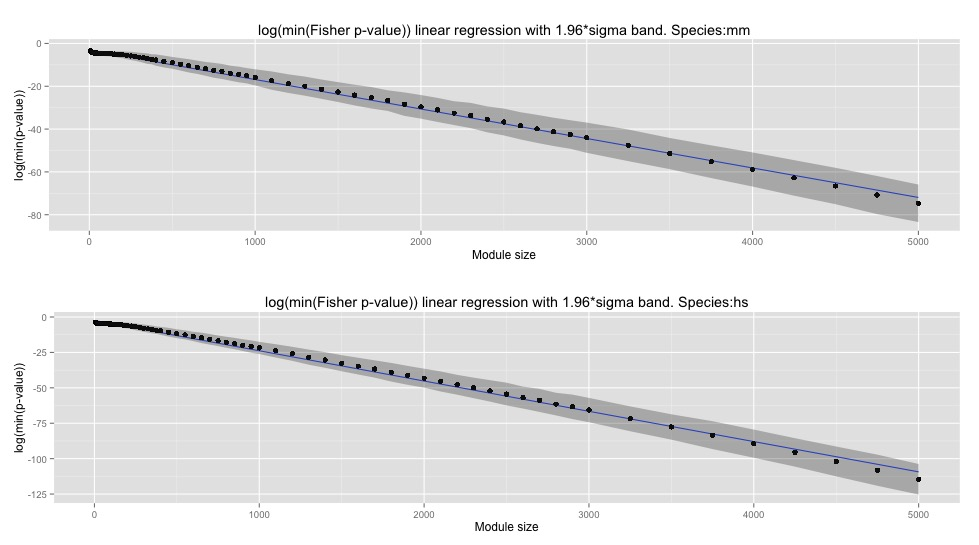
\includegraphics[width=\textwidth]{./img/mean_linear_regression_with_confidence.jpeg}
    \end{figure}
\end{frame}

\begin{frame}{Adjusted $p_{value}$}
  \begin{itemize}[<+->]
    \item Пусть поступил запрос длины $n$, и для всех модулей вычислена значимость $p_i$
    \item Из уравнений регрессий получим значения $mean$ и $std$
    \item Построим нормальное распределение $\mathcal{N}(mean, std)$
    \item Для каждого $p_i$ посчитаем $p^{adj}_i = CDF(p_i) = \mathsf{Pr}(X \le p_i)$ 
        \begin{figure}[!ht]
        \centering
        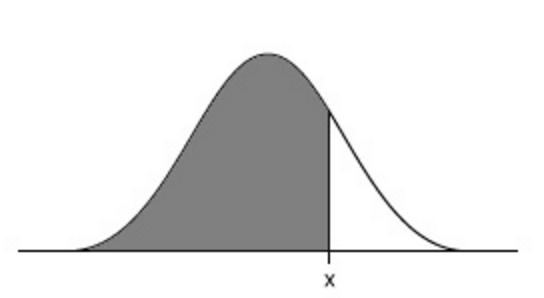
\includegraphics[width=0.4\textwidth]{./img/bell.png}
    \end{figure}
  \end{itemize}
\end{frame}

\begin{frame}{Формирование выдачи}
  \begin{itemize}[<+->]
    \item Оставим только те модули, для которых $p^{adj} \le 0.01$
    \item Отсортируем модули по возрастанию $log(p^{adj})$
        \begin{figure}[!ht]
            \centering
            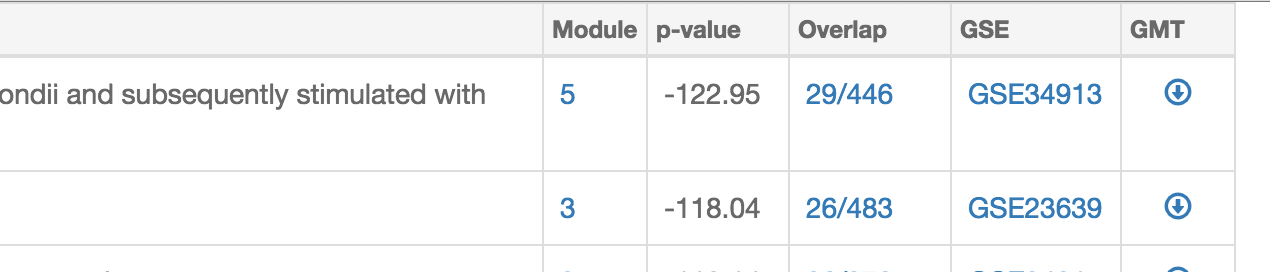
\includegraphics[width=\textwidth]{./img/screen_p_value.png}
        \end{figure}
  \end{itemize}
\end{frame}

\subsection{Тонкости реализации}

\begin{frame}{Общая информация}
  \begin{itemize}[<+->]
    \item Веб-сервис реализован на Python/Django/ReactJS/Java
    \item PostreSQL
    \item Ресурсоемкие вычисления происходят на Java
  \end{itemize}
\end{frame}

\begin{frame}{Скорость вычислений}
  \begin{itemize}[<+->]
    \item Обработка запроса $=$ нахождение $\sim$ 50k пересечений запроса размера $n$ с каждым модулем размера $m_i$
    \item Нужны \emph{все} модули для вычисления результата
    \item Считывание всех модулей каждый раз из БД --- долго (около 40 сек на запрос) и нагружает БД
  \end{itemize}
\end{frame}

\begin{frame}{Оптимизации}
  \begin{itemize}[<+->]
    \item Вычислительный сервер на Java
    \item Храним данные в оперативной памяти
    \item Используем примитивные типы данных: \sout{List<Double>} double[]
    \item Храним модули отсортированными, чтобы пересекать их с запросом за $O(\mathsf{min}(m_i, n))$
    \item Профит! ($\sim$ 3 сек на запрос)
  \end{itemize}
\end{frame}


\section{Уточнение модели}

\begin{frame}{Распределение частот генов в базе GeneQuery}
    \begin{itemize}[<+->]
	    \item Для каждого гена $g_i$ посчитаем количество вхождений в БД $freq(g_i)$
	    \item Это равно количеству GSE, в которых ген себя «проявил»
	    \item Занумеруем гены по невозрастанию их частот: $i \ge j \Rightarrow freq(g_i) \le freq(g_j)$
	    \item Определим вероятность появления гена: 
	        $$p(g_i) = \frac{freq(g_i)}{\sum\limits_{j}{freq(g_j)}} = \frac{freq(g_i)}{\sum\limits_{m \in Modules}{length(m)}}$$
	 \end{itemize}
\end{frame}

\begin{frame}{Распределение частот генов в базе GeneQuery}
    \begin{figure}[p]
        \centering
        \caption{Зависимость частоты гена от его номера.}
        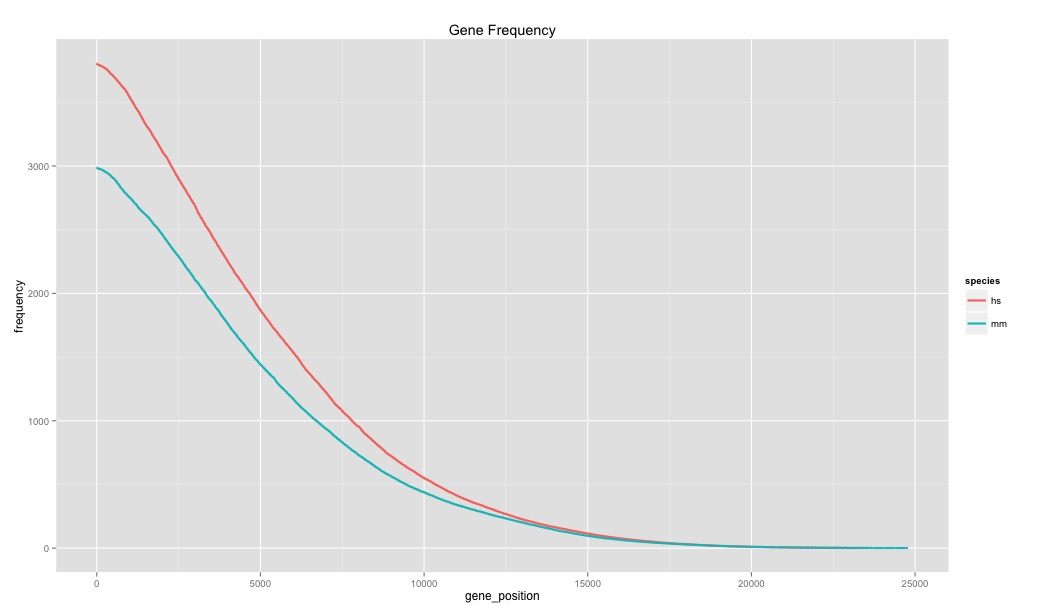
\includegraphics[height=0.8\textheight]{./img/gene_position_to_freq.jpeg}
    \end{figure}
\end{frame}

\begin{frame}{Распределение частот генов в базе GeneQuery}
    \begin{figure}[p]
        \centering
        \caption{Плотность распределения частот генов для мыши.}
        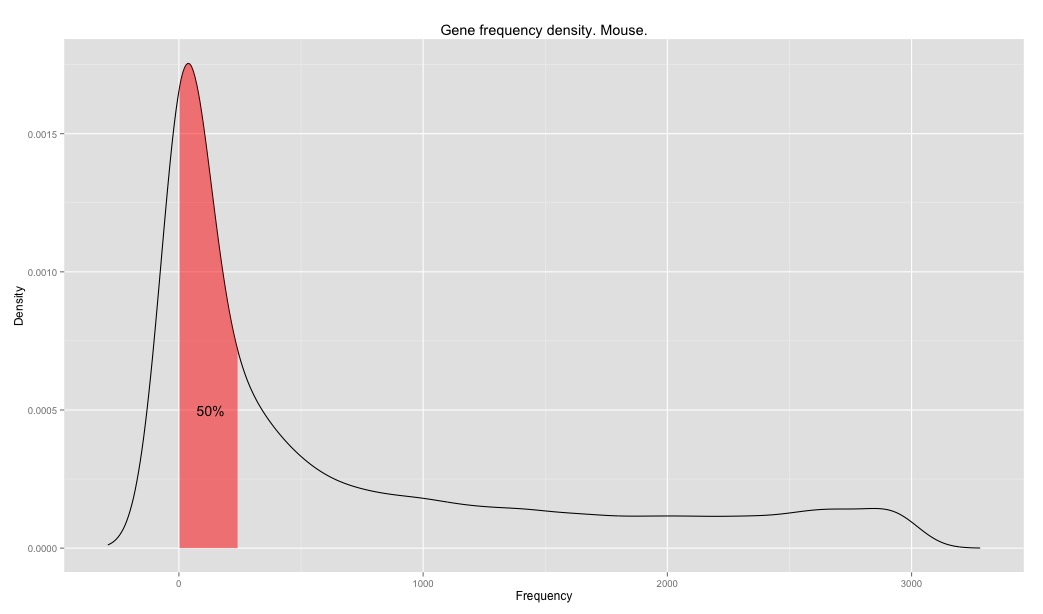
\includegraphics[height=0.8\textheight]{./img/gene_freq_density_mm.jpeg}
    \end{figure}
\end{frame}

\begin{frame}{Bootstrapping для разных страт}
    \begin{itemize}[<+->]
	    \item \emph{Страта} --- набор генов с частотами в определенном интервале
	    \item Разделим множество генов на страты 1-1000, 1000-2000, 2000-3000 и 3000-4000 (последний только для человека)
	    \item Bootstrapping для каждой страты
	    \item Построим регрессию $log(\mathsf{min}(p_{value})) \sim \mathsf{size}$
	 \end{itemize}
\end{frame}

\begin{frame}{Bootstrapping для страт}
    \begin{figure}[ht]
        \centering
        \caption{Регрессии для страт (первая страта --- из самых частых генов).}
        \includegraphics[height=0.75\textheight]{./img/mean_regression_all_strats_compare.jpeg}
    \end{figure}
\end{frame}

\begin{frame}
    \begin{figure}[p]
        \centering
        
\includegraphics[width=0.5\textwidth]{./img/wut.jpeg}
    \end{figure}
\end{frame}

\begin{frame}{Резюмируем проблему}
    \begin{itemize}[<+->]
	    \item Частые гены «искусственно» увеличивают значимость пересечения
	    \item Хочется учитывать частоту гена при вычислении значимости (т.е. ранжировании результатов)
	    \item В идеале регрессия не должна зависеть от частот генов из запросов
	 \end{itemize}
\end{frame}

\begin{frame}{Идея решения: начальные условия}
    \begin{itemize}[<+->]
	    \item Распределение частот в БД \emph{не является моделью «внешнего мира»}
	    \item Гены в запросе \emph{независимы в совокупности}
	 \end{itemize}
\end{frame}

\begin{frame}{Идея решения: общий вид}
    Для фиксированного модуля и запроса:
    \begin{equation}
        f(p_{value}(I)) \cdot w(I)
    \end{equation}
    \begin{description}
        \item $I = (g_1, g_2, \dots, g_n)$ --- пересечение генов модуля и запроса
        \item $f(I)$ --- некая функция от $p_{value}$ (логарифм в нашем случае), полученного точным тестом Фишера (не учитывает распределение генов)
        \item $w(I)$ --- некая функция, зависящая от распределения генов из $I$, отражающая \alert<2>{«информативность»} пересечения
    \end{description}
\end{frame}

\begin{frame}{Информативность}
    \begin{itemize}[<+->]
        \item Пусть имеется некий набор генов
	    \item Интуитивно: \emph{чем больше частых генов в наборе, тем меньше информативность всего набора}
	    \item Как это записать аналитически?
	    \item Энтропия
	 \end{itemize}
\end{frame}

\begin{frame}{Энтропия}
    \begin{itemize}[<+->]
        \item Мера информации: чем больше энтропия, тем меньше информации
        \item Энтропия гена:
            $$\mathcal{H}(g) = -p(g) log(p(g))$$
	    \item Энтропия набора генов:
	        $$\mathcal{H}(I) = \sum\limits_{g \in I}{\mathcal{H}(g)} = \sum\limits_{g \in I}{-p(g) log(p(g))}$$,
	        так как гены из $I$ независимы в совокупности
	    \item Общий вид функции информативности:
	        $$w(I) \sim \hat{w}(\frac{1}{\mathcal{H}(I)})$$,
	        чем больше редких генов в $I$, тем меньше энтропия, тем больше значение функции
	 \end{itemize}
\end{frame}

\begin{frame}{Общий вид значимости пересечения}
    \begin{equation}
        f(p_{value}(I)) \cdot w(I) = f(p_{value}(I)) \cdot \hat{w}(\frac{1}{\mathcal{H}(I)})
    \end{equation}
    где $\hat{w}$ монотонно не убывает
\end{frame}

\begin{frame}{Интерпретация новой значимости}
    \begin{itemize}[<+->]
        \item (значимость получить пересечение заданного размера) $\times$ (значимость генов внутри пересечения)
	    \item Подбор вида функции $\hat{w}$ так, чтобы компенсировать расхождения из-за частот генов
	    \item Значения новой значимости должны иметь параметрическое распределение (или приближаться им)
	 \end{itemize}
\end{frame}

\section{Аннотация генов}

\begin{frame}{Аннотация генов}
  \begin{itemize}[<+->]
    \item Существует множество GPL платформ для аннотации генов
    \item Ген аннотируется в один или несколько id разных видов (Symbol, Ensembl, etc)
    \item Нет уникального соответствия между разными видами id
    \item Entrez --- натуральное число, уникальное для \emph{каждого} гена среди \emph{всех} организмов
  \end{itemize}
\end{frame}

\begin{frame}
    \begin{figure}[!ht]
        \centering
        \caption{Conversion flow.}
        \includegraphics[height=0.9\textheight]{./img/conversion.png}
    \end{figure}
\end{frame}

\begin{frame}{Детализация конвертации в GeneQuery}
    \begin{figure}[p]
        \centering
        \caption{Детализация конвертации генов.}
        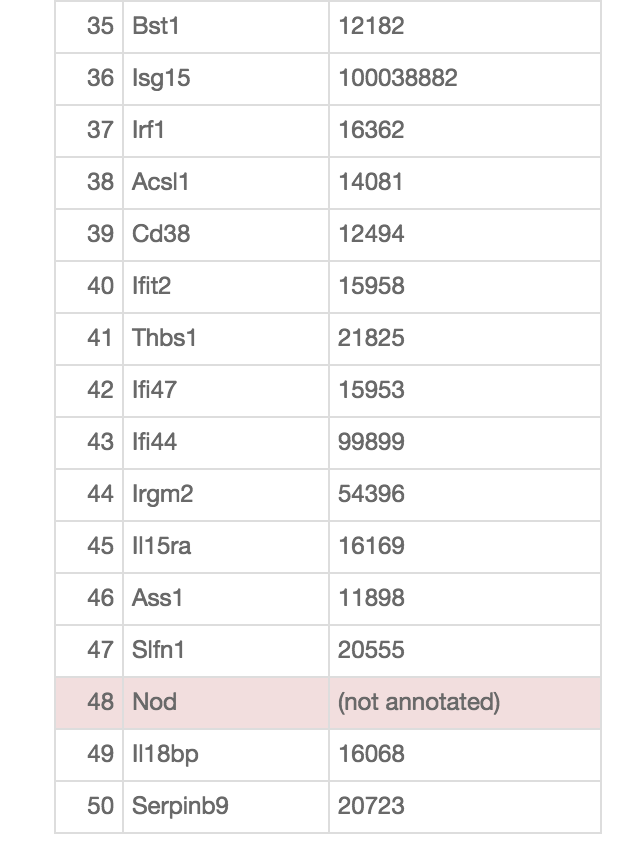
\includegraphics[height=0.8\textheight]{./img/screen_details.png}
    \end{figure}
\end{frame}


\section{Ортология}

\begin{frame}{Что это и зачем}
  \begin{itemize}[<+->]
    \item \emph{Ортология} --- раздел генетики, изучающий свойства генов разных особей, происшедших от одного общего предка
    \item Хочется искать модули одного организма по генам другого
    \item Указываем организм запроса и организм области поиска
        \begin{figure}[!ht]
            \centering
            \includegraphics[width=0.6\textwidth]{./img/screen_query_orthology.png}
        \end{figure}
  \end{itemize}
\end{frame}

\begin{frame}{Homology}
    \begin{figure}[p]
        \centering
        \caption{Трансляция генов разных организмов.}
        \includegraphics[height=0.8\textheight]{./img/homology_diagramm.png}
    \end{figure}
\end{frame}

\begin{frame}{Homology в GeneQuery}
    \begin{figure}[p]
        \centering
        \caption{Общий вид трансляции генов разных организмов.}
        \includegraphics[height=0.8\textheight]{./img/homology.png}
    \end{figure}
\end{frame}



\plain{Вопросы?}

\end{document}
